\documentclass[12pt, english, twoside]{article} %twoside necessary for fancyheader odd vs. even commands 

\usepackage[letterpaper]{geometry}
%\geometry{verbose, a4paper, tmargin=1in,bmargin=1in,lmargin=1.25in,rmargin=1.25in}
\geometry{verbose, a4paper, tmargin=3cm,bmargin=3cm,lmargin=3cm,rmargin=3cm} 

\usepackage{amsmath, hyperref, enumerate, comment}
\usepackage{amsfonts, esint, setspace}
\usepackage{graphicx}
\usepackage{mathrsfs} %for script font 

\linespread{1.3}	

\raggedbottom % prevents random spaces between paragraphs from appearing

\usepackage[titletoc,title]{appendix}

% headers
\usepackage{fancyhdr} 
\pagestyle{fancy}
\fancyhead{}
\fancyhead[OR,ER]{\large \textbf{\thepage}}
%\fancyhead[C]{\textit{}}% odd page header and number to right top
%\fancyhead[EC]{\textit{Your Name}}%Even page header and number at left top
\fancyfoot[L,R,C]{}
\renewcommand{\headrulewidth}{0pt}
%\renewcommand{\footrulewidth}{0pt}
\renewcommand*\footnoterule{} %removes footnote line


% % redefines abstract to be capitalized, with no margins 
\renewenvironment{abstract}
 {\small
  \begin{center}
\normalsize  \textnormal{ABSTRACT\\} \vspace{-0em}\vspace{0pt}
  \end{center}
  \list{}{%
    \setlength{\leftmargin}{0in}%
    \setlength{\rightmargin}{\leftmargin}%
  }%
  \item\relax}
 {\endlist}

% section headings
\usepackage{sectsty}
\allsectionsfont{\large\raggedright\centering}

% Table of contents stuff and footnotes 
\setcounter{tocdepth}{2}
\usepackage[]{tocloft}
%\addtocontents{toc}{\cftpagenumbersoff{section}} % turns off page numbers from section level 
%\addtocontents{toc}{\cftpagenumbersoff{subsection}} %like wise for subsection level 
\renewcommand{\cftsecfont}{\itshape}
\renewcommand{\cftsubsecfont}{\itshape}
\renewcommand{\cftsecpresnum}{\normalfont \bfseries} % puts the section numbers in non-italics and bold
\renewcommand{\cftsubsecpresnum}{\normalfont \bfseries} % likewise for subsection numbers 

\renewcommand{\cftbeforesecskip}{3pt} %controls spacing between ToC items 
\makeatletter
\renewcommand{\@cftmaketoctitle}{}

% % footnote modification: must be between \makeatletter and \makeatother

\renewcommand{\@makefntext}[1]{%
  \setlength{\parindent}{0pt}%
  \begin{list}{}{\setlength{\labelwidth}{6mm}% indents footnote text 
    \setlength{\leftmargin}{\labelwidth}%
    \setlength{\labelsep}{5pt}% moves footnote mark to the left
     \setlength{\itemsep}{0pt}%
      \setlength{\parsep}{0pt}%
      \setlength{\topsep}{-3pt}% removes separation between footnotes
    \footnotesize}%
  \item[\@textsuperscript{\@thefnmark}\hfil ]#1% @makefnmark
  \end{list}%
}
%      \setlength{\footnotesep}{0pt}%

\makeatother
\renewcommand{\cftdot}{} % removes dots from table of contents 


% % for fonts:
\usepackage[T1]{fontenc}
\usepackage[utf8]{inputenc}
\usepackage{mathptmx}
%\usepackage{mathpazo}

% Hyperref set-up & metadata
\hypersetup{
	pdftitle={Your Paper Title},
	pdfauthor={Your Name},
	pdfsubject={},
	pdfkeywords={},
	pdfcreator={XeLaTeX},
	pdfproducer={XeLaTeX},
	pdftoolbar=false,	% show Acrobat’s toolbar?
	pdfmenubar=true,	% show Acrobat’s menu?
	pdffitwindow=false,	% window fit to page when opened
	pdfstartview={FitH},	% fits the width of the page to the window
	unicode=true,		% non-Latin characters in Acrobat’s bookmarks
	pdfnewwindow=true,	% links in new window
	colorlinks=true,	% false: boxed links; true: colored links
	linkcolor=black,	% color of internal links
	citecolor=black,	% color of links to bibliography
	filecolor=black,	% color of file links
	urlcolor=blue		% color of external links
}


%\usepackage[backend=biber, style=authoryear, url=false, doi=false, eprint=false]{biblatex}




% % % Biblatex commands for Citations and References:
\usepackage[backend=biber, style=ext-authoryear-comp,  maxcitenames=2, dashed=false, url=false, doi=false, eprint=true, giveninits=true, innamebeforetitle=true, maxbibnames=6]{biblatex} 

\addbibresource{bibliography.bib}

%\addbibresource{templateReferences.bib} %%generated by reference items above
%maxcitenames=2 replaces all instances of more than 2 authors in citations with `et al.', but lists all authors in references
%labeltitleyear=true; sortcites=true
%innamebeforetitle=true places editors before the book titles
%style=authoryear-comp adds in some weird ``In:'' stuff in reference list that must be changed below. 

%\DeclareFieldFormat{labeldate}{\mkbibbrackets{#1}} %puts brackets around years in citations

\DeclareFieldFormat{postnote}{\mkpageprefix[pagination][\mkcomprange]{#1}} % compresses page range in citations, so that unchanged digits are not repeated. See p. 259, section 4.6.4 of biblatex manual.  %also adds pagination prefix p.

% clears un-needed fields from reference items
\AtEveryBibitem{%
 \clearfield{note}%
  \clearfield{series}%
 \clearfield{number}%
 \clearfield{pagetotal}%
 \clearfield{chapter}%
  }
  %\clearfield{pages}%}
  
  
  \renewcommand{\newunitpunct}{\addcomma\space} %makes a comma the default separator between items; overridden in some cases by commands below

\renewcommand{\intitlepunct}{\addspace\nopunct} %removes punctuation after ``in"

\DeclareDelimFormat[bib,biblist]{nametitledelim}{\addcolon\space} %puts colon after year

%\DeclareFieldFormat{biblabeldate}{\mkbibbrackets{#1}} %puts brackets around years in references

\DeclareFieldFormat{editortype}{\mkbibparens{\textit{#1}}} %puts ed in parentheses
\DeclareDelimFormat{editortypedelim}{\addspace}%prevents punctuaction clash after (ed)
\DeclareDelimFormat[bib,biblist]{innametitledelim}{\addcomma\space} % puts comma after (ed)

\DeclareFieldFormat{eprint}{\printtext{available at}\addspace \textless#1\textgreater} % Calls url from Eprint field. See biblatex manual, section 4.11.2 Electronic Publishing Information, page 310-11
  
\DeclareFieldFormat[article,periodical]{volume}{\textbf{#1}} %puts volume in bold; note that adding \bibstring{jourvol}~ before #1} prints ``vol.". from biblatex-ext manual 
%\DeclareFieldFormat[article,periodical]{number}{#1}%\bibstring{number}~ before #1} prints ``vol."
\renewcommand*{\jourvoldelim}{\addcomma\space} %combined with above command, puts comma after article title and before journal volume. 
%\renewcommand*{\volnumdelim}{\addcomma\space}

\DeclareFieldFormat[inbook, incollection, book]{volume}{\bibcpstring{volume}~#1} %capitalizes `Vol' after book titles. 

\DeclareFieldFormat{pages}{\mkpageprefix[pagination][\mkcomprange]{#1}} % compresses page range in bibliography, so that unchanged digits are not repeated. 

% % following command suppresses ``in" for articles and inproceedings only
\renewbibmacro{in:}{%
\ifboolexpr{%
test {\ifentrytype{article}}%
or
test {\ifentrytype{inproceedings}}%
}
{}%<-nothing
{\printtext{\bibstring{in}\intitlepunct}}%<-normal ’in’ with punctuation
}


\newcommand{\diff}{\mathop{}\!\mathrm{d}} %defines exterior derivative 
\renewcommand{\div}[1]{\gv{\nabla} \cdot #1} % for divergence
\newcommand{\curl}[1]{\gv{\nabla} \times #1} % for curl
\renewcommand{\vector}[1]{\ensuremath{\vec{#1}}} % redefines vector to vec
\newcommand{\integral}{\int}

\newcommand\bs{\begin{singlespace}} 			
\newcommand\es{\end{singlespace}} 	


\begin{document}

\title{\vspace{-3em} \LARGE Hamiltonian Privilege }			
%\author{\Large \textsuperscript{*\textdagger}}
\date{\vspace{-7.9ex} \today}
\maketitle
%
\vspace{-8mm}

\noindent\rule{\textwidth}{1.25pt}
\bs
\noindent {\normalsize We argue that Hamiltonian mechanics is more fundamental than Lagrangian mechanics. Our argument provides a non-metaphysical strategy for privileging one formulation of a theory over another: a formulation is more fundamental when it is more general. We illustrate this criterion through a novel interpretation of classical mechanics, based on three physical conditions. Two of these conditions suffice for recovering Hamiltonian mechanics. A third condition is necessary for Lagrangian mechanics. Hence, Lagrangian systems are a proper subset of Hamiltonian systems. Finally, we provide a geometric interpretation of the principle of stationary action and rebut arguments for privileging Lagrangian mechanics. }
\es
\noindent\rule{\textwidth}{1.25pt}

%\vspace{2mm}

\bs
\tableofcontents 
\es


\section{Introduction}
\label{introduction}


The intellectual richness of classical mechanics manifests itself in an abundance of formulations, with Newtonian, Hamiltonian, Lagrangian, and Hamilton--Jacobi being among the most prominent.  Butterfield \parencites*[]{Butterfield2004} has aptly referred to these formulations as different \textit{schemes} for treating classical systems. Recent work in philosophy of science has focused largely on how these schemes relate to one another, with the aim of arriving at a deeper understanding of classical mechanics. By considering the conceptual differences between these formulations, we can better interpret the physical significance of our representations.

In the context of comparing Hamiltonian and Lagrangian mechanics, three interpretive stances have emerged. \textcites[]{North} has argued for privileging Hamiltonian mechanics on the grounds that it requires less mathematical structure to formulate. In contrast, \textcites[]{Curiel} recommends privileging Lagrangian mechanics, arguing that it isolates physically-significant kinematical constraints that all classical systems must satisfy. Finally, we can interpret Lagrangian and Hamiltonian mechanics as theoretically equivalent in a precise mathematical sense. Within a subclass of systems known as the \textit{hyper-regular domain}, the two formalisms are categorically equivalent \parencites[]{Teh}{Barrett2}. Categorical equivalence provides a natural interpretive criterion for theoretical equivalence because it yields mutual inter-translatability between theory formulations. This equivalence motivates the view that there are no physically significant differences between these two formalisms, at least within the hyper-regular domain. 

Here, we will argue that there are indeed physical grounds for privileging Hamiltonian mechanics over Lagrangian mechanics, their categorical equivalence notwithstanding.\footnote{Barrett shows that in the hyper-regular domain, Lagrangian and Hamiltonian mechanics are categorically equivalent provided that we define categories of models over the tangent and cotangent bundle formulations, respectively \parencites*[1181-82]{Barrett2}. However, he also shows that if we consider a more general formulation of Hamiltonian mechanics on a symplectic manifold (which does not require a cotangent bundle), then the two formulations are \textit{not} categorically equivalent \parencites*[1182-83]{Barrett2}. Our construction of Hamiltonian mechanics in Section~\ref{derivation} matches this more general symplectic manifold formulation.} Whereas North's argument relies on a problematic criterion for comparing structure based on the size of symmetry groups \parencites[]{Swanson}, our argument avoids this pitfall. We show that a classical system needs to satisfy strictly fewer physical conditions in order to be Hamiltonian. To be Lagrangian, systems must satisfy an additional physical condition, making Lagrangian mechanics a proper subset of Hamiltonian mechanics. Hamiltonian mechanics thereby captures a wider range of systems than Lagrangian mechanics, and this difference has interpretive consequences even within the hyper-regular domain. The construction at the heart of our argument provides an interpretation of classical mechanical systems in terms of their invariant phase space density. 
%We show that the invariant density fits more naturally within the Hamiltonian framework, providing another reason to privilege it over Lagrangian mechanics.
% Our formalism also provides a novel interpretation of the principle of stationary action within Hamiltonian mechanics.

Section~\ref{privileging} previews our argument for privileging Hamiltonian mechanics. We introduce three physical conditions that define classical systems while distinguishing Hamiltonian from Lagrangian mechanics. Section~\ref{fundamentality} explains how our position differs from North's. Specifically, our argument does not require metaphysical commitments to fundamental structure or perfectly natural properties. Section~\ref{derivation} describes in detail the derivation of Hamiltonian mechanics for systems that satisfy two physical conditions: infinitesimal reducibility and deterministic/reversible evolution. We then show that Lagrangian systems must satisfy an additional physical condition, which we call motion equivalence. This completes our primary argument for privileging Hamiltonian mechanics. Section~\ref{Lagrangian} considers the status of Lagrangian mechanics within our framework. We provide a geometric interpretation of the action principle, which applies even outside the hyper-regular domain. We end by rebutting objections that arise from Curiel's \parencites*[]{Curiel} privileging of Lagrangian mechanics. 




\section{Privileging Hamiltonian mechanics}
\label{privileging}

In claiming that Hamiltonian mechanics is more fundamental than Lagrangian mechanics, we must clarify what we mean by ``fundamental.'' Of various notions of fundamentality, we mean something entirely non-mysterious. Given two formalisms that capture a class of systems, if one is logically more general, then it is conceptually more fundamental. Conceptual fundamentality is familiar from mathematics. A more fundamental framework encompasses a less fundamental one as a special case. It is in this sense that the generalized Stokes' theorem is more fundamental than well-known special cases, such as the fundamental theorem of calculus and Green's theorem. Similarly, an axiomatization which includes additional axioms is less fundamental than one which drops these axioms while maintaining the same expressive power. Conceptual fundamentality is distinct from notions of fundamentality associated with differences in energy scale, such as how the Standard Model of particle physics is more fundamental than classical mechanics. We do not mean that Hamiltonian mechanics is more fundamental than Lagrangian mechanics in this sense.
%\footnote{In Section~\ref{density}, we embrace a related non-metaphysical notion of fundamentality that pertains to physical entities rather than theoretical frameworks.} 

To apply our criterion for fundamentality, we must show that Lagrangian mechanics is less general than Hamiltonian mechanics. We do this in Section~\ref{derivation} by recovering the mathematical formalisms of both Hamiltonian and Lagrangian mechanics from three physical conditions. Our aim here is to show how this argument works in principle. Section~\ref{fundamentality} demonstrates some philosophical advantages of our preferred notion of fundamentality.\footnote{One might worry that our criterion for fundamentality is subject to elementary counterexamples. For instance, can't we make any theory more general by adjoining arbitrary disjunctions? Importantly, we require that the theory remains wholly \textit{about} classical mechanics. Hamiltonian mechanics is more general than Lagrangian mechanics while still being about classical systems, where ``aboutness'' can be understood using Yablo's framework \parencites*[]{Yablo}. Having an account of \textit{aboutness} or \textit{subject matter} is a general philosophical problem that any account of fundamentality must address. It is not a special problem facing our criterion.} 
%We will show that the Lagrangian framework is less general because it requires an additional condition to hold, compared to the Hamiltonian framework. Hence, the Lagrangian framework is less fundamental because it is a proper subset of the Hamiltonian framework.

%We will, however in Section 5 give a criterion for an entity to be physically fundamental
%These bolster our claim that this is an appropriate sense of fundamentality for philosophers to focus on. 

% From Healey 2007, (weak) separability says that ``any physical process occupying space-time region R supervenes upon an assignment of qualitative intrinsic physical properties at space-time points in R (and/or in arbitrarily small neighborhoods of those points)'' [46]
% Non-separability: ``some physical process occupying a region R of space-time is not supervenient upon an assignment of qualitative intrinsic physical properties at space-time points in R'' [124]
% Strong non-separability: ``some physical process occupying a region R of space-time is not supervenient upon an assignment of qualitative intrinsic physical properties at points of R and/or in arbitrarily small neighborhoods of those points'' [124].

Shorn of many details, our argument goes as follows. First, we show that the formalism of Hamiltonian mechanics applies to systems that are both i) infinitesimally reducible and ii) follow a deterministic and reversible evolution. A system is \textit{infinitesimally reducible} provided that the state of the whole system is equivalent to specifying the states of its parts (and vice versa). Colloquially, we can say that the whole state equals the sum of its parts, where we take these infinitesimal parts to be classical particles. Infinitesimal reducibility distinguishes classical from quantum systems, where the latter are irreducible (i.e. we cannot specify the whole state by specifying the states of its subsystems).\footnote{The conditions of infinitesimal (ir)reducibility are similar to various notions of (non-)separability in the literature on physical holism \parencites[46, 124]{Healey}. We adopt our preferred terminology to avoid controversies surrounding how best to characterize separability.} We show in Section~\ref{infinitesimal} that the phase space of infinitesimally reducible systems must have at least the structure of a symplectic manifold. Recovering Hamiltonian mechanics then simply requires identifying when trajectories on phase space obey Hamiltonian evolution  (i.e. evolve according to a symplectomorphism). Section~\ref{deterministic} shows that this requires the system to follow a \textit{deterministic and reversible evolution}, i.e. the present state of the system uniquely determines both its future and past states. We thereby characterize Hamiltonian mechanics as the mathematical framework for infinitesimally reducible systems with deterministic and reversible evolution.  
%Since we won't have to settle controversies surrounding these terms, we adopt our preferred terminology.

Next, we note that some classical systems satisfy a third, further condition, which we call \textit{motion equivalence}. Motion equivalence holds when the system's trajectory in physical space determines---and is determined by---its evolution in phase space. In other words, knowledge of the trajectory in physical space (e.g. Euclidean three-space $\mathbb{R}^3$) suffices for knowledge of the trajectory in phase space, and vice versa. Physically, knowledge of the trajectory in physical space corresponds to knowledge of position and velocity, while knowledge of the trajectory in phase space requires knowing the system's momentum. Hence, motion equivalence entails a correspondence between velocity and momentum, which formally leads to the framework of Lagrangian mechanics in the hyper-regular domain (Section~\ref{motion}). As a result, Lagrangian mechanics requires that a further physical condition is satisfied, and hence it is less general than Hamiltonian mechanics. 

To show that motion equivalence is a further condition, it suffices to show that some Hamiltonian systems violate it. This follows from the fact that knowing a system's position and velocity does not always suffice for knowing its momentum. Hence, we cannot always determine the evolution of a system in phase space from its trajectory in physical space. For instance, if we consider a photon as a classical particle, then we cannot determine its momentum from its trajectory through space. Since photons travel at constant speed, we can recover the direction of momentum---but not the magnitude---from the trajectory. Two photons with different momenta can follow the same trajectory in physical space. Hence, knowledge of the physical trajectory of a photon is insufficient for knowledge of its phase space evolution. In general, different Lagrangians---differing even by more than a constant---can correspond to the same particle trajectories while not agreeing on the total energy, even up to a constant.\footnote{\textcites[1185--1186]{Barrett2} discusses this in the context of the failure of equivalence between the vector field formulations of Lagrangian and Hamiltonian mechanics. In contrast, the trajectories in phase space (encoded by the Hamiltonian vector field) uniquely define the Hamiltonian up to a constant.} Hence, the set of classical systems that satisfy motion equivalence is a proper subset of the classical systems that satisfy the conditions for Hamiltonian mechanics. For at least this reason, Hamiltonian mechanics is more fundamental than Lagrangian mechanics.

% % optional: address refer 1 concern about the clarity of this argument/example: ``what if momentum is defined in terms of velocity? Or is the idea to know that we also need to know the mass?"

Of course, different definitions of ``Hamiltonian'' and ``Lagrangian'' systems can result in different interpretive relationships. On our account, Hamiltonian systems are infinitesimally reducible and follow deterministic and reversible evolution.\footnote{Although not sufficient for a definition, Newtonian systems also satisfy the motion equivalence assumption. Since Lagrangian systems satisfy all three conditions (infinitesimal reducibility, deterministic/reversible evolution, and motion equivalence), they lie in the intersection of Newtonian and Hamiltonian systems.} We thereby set aside well-known cases of non-deterministic classical systems.\footnote{For discussion of non-deterministic classical systems, see \textcites*[3-4]{Baez}{Earman}{Norton}.} Additionally, we set aside dissipative systems, i.e. those that fail to conserve energy. Possessing a deterministic and reversible evolution is equivalent to being non-dissipative. Our derivation of Lagrangian mechanics in Section~\ref{motion} takes place within the context of conservative systems, so we do not consider systems that satisfy inhomogenous Euler--Lagrange equations. Although both the Lagrangian and Hamiltonian formulations apply to dissipative systems, we exclude these.\footnote{For details, see \textcites[\S 10.4]{Cline}. Curiel \parencites*[311]{Curiel} acknowledges that the Hamiltonian framework can be extended to treat dissipative systems. For details of a Lagrangian approach to dissipative systems, see \textcites[]{Smith}.} This restricts our claim about the fundamentality of Hamiltonian mechanics to the non-dissipative regime. Finally, our treatment is not restricted to $n$-particle mechanics but applies as well to rigid-body and continuum mechanics. This supports our claim that the property of infinitesimal reducibility fruitfully characterizes classical systems. Before presenting the details of our argument in Section~\ref{derivation}, we describe how we avoid central problems facing North's privileging of Hamiltonian mechanics. 
%, although Curiel seems to view it as a virtue of the Lagrangian formulation that it handles dissipative systems with fewer modifications.


\section{Fundamentality, \textit{sans} metaphysics}
\label{fundamentality}

As indicated at the start of Section~\ref{privileging}, we use ``fundamentality'' in a non-metaphysical sense. Some differences in fundamentality are differences in generality: provided a theoretical framework still captures the relevant behavior, it is more fundamental if it requires fewer conditions to hold. Our notion of fundamentality leads to a correspondingly non-metaphysical notion of ``structure.'' Hamiltonian mechanics employs less structure than Lagrangian mechanics because the former requires fewer physical conditions. Compared with North's \parencites*[]{North} account of structure, our definition has two advantages. First, it avoids metaphysical disputes surrounding perfectly natural or joint-carving properties, which scientific anti-realists and pragmatists decry. Secondly, it avoids a technical objection that Swanson and Halvorson \parencites*[]{Swanson} levy against North's more precise mathematical criterion for comparing structure. 

Despite our different commitments, our approach has methodological parallels to North's. We agree with North that it is fruitful to identify both invariants and ``the mathematical structure needed to formulate the theory in an invariant, frame-independent way'' \parencites*[65]{North}. Additionally, we agree that it is worthwhile to identify what particular mathematical structure is required by a formulation \parencites[78]{North}. Indeed, we undertake precisely this sort of investigation in Section~\ref{derivation}.\footnote{Curiel also aims to identify the necessary and sufficient mathematical structures for formulating classical mechanics. He sets out to establish the ``geometrical structure necessary (and manifestly sufficient) for the formulation of the Euler--Lagrange equation'' relevant for all kinematically-possible solutions \parencites*[292]{Curiel}. See Section~\ref{Curiel} for discussion.} However, North advocates a metaphysical account of structure, about which we remain agnostic. According to North, ``structure comprises the objective, fundamental, intrinsic features, the ones that remain the same regardless of arbitrary or conventional choices and description'' \parencites*[66]{North}. These notions of fundamentality and intrinsicality correspond to differences in joint-carving, where more fundamental or intrinsic features are more joint-carving (or in Lewis's \parencites*[]{Lewis1983} terminology, more natural). 

Owing to the epistemic difficulty of accessing these putative joints, we do not endorse these metaphysical dimensions of structure or fundamentality.\footnote{For a detailed discussion of difficulties facing the notion of metaphysical naturalness, see \textcites[]{Dorr_Hawthorne}.} While Hamiltonian mechanics is significant partly because it elucidates invariant densities, this does not entail that additional mathematical structure is physically insignificant or surplus. Additional structure may correspond to an additional physically-significant assumption that applies to the system under consideration. Precisely this scenario occurs in the context of Lagrangian mechanics, which requires the additional condition of motion equivalence to hold. Whereas North views Lagrangian mechanics as containing ``excess, superfluous structure'' \parencites*[75]{North}, we take this additional condition as optional but still physically significant. Thus, while it is illuminating to identify the minimum mathematical structures necessary for a formulation, additional structure is not automatically rendered physically insignificant. 

Additionally, whereas North \parencites*[76]{North} seeks to determine the ``real'' fundamental state space structure of the theory---and correspondingly, of a classical world---we remain neutral on this underlying metaphysical question.\footnote{Indeed, Swanson and Halvorson \parencites*[]{Swanson} note that many physicists and philosophers would not interpret statespace structure ontologically, but as a formal device for encoding physical information or a calculational tool. As Wilson illustrates, we can interpret classical mechanics while avoiding---and even rejecting---the search for what is ``fundamental in the bottom-layer sense'' \parencites*[53]{Wilson}.} Whether Hamiltonian phase space structure is metaphysically fundamental in a classical world does not matter for the questions we seek to answer. Regardless of its metaphysical status, Hamiltonian mechanics is conceptually more fundamental. Indeed, our argument does not privilege any one of the various mathematical formalizations of Hamiltonian mechanics. These include formulating Hamiltonian mechanics on a $2n+1$-dimensional contact manifold, on an extended phase space, on a Poisson manifold, and the standard formulation on a symplectic manifold that we recover in Section~\ref{deterministic}.\footnote{Tulczyjew's reformulation of Hamiltonian mechanics further supports viewing symplectic geometry---and hence Hamiltonian mechanics---as conceptually fundamental. According to Teh and Tsementzis, this reformulation shows that  ``the very concept of a classical mechanical system (and not merely the phase space of that system) should be described in terms of symplectic geometry'' \parencites*[46]{Teh}.}

North also introduces a technical notion of comparative structure, based on the symmetry group of statespace. According to this criterion, statespace A has more structure than statespace B if the symmetry group of A is a proper subgroup of B's symmetry group \parencites[87-88]{North}.\footnote{This criterion follows from the most charitable reconstruction of North's argument, given by \textcites[]{Swanson}. North sometimes speaks in terms of comparing the dimensions of symmetry groups, which they note leads to counterexamples.} Being a proper subgroup entails that strictly fewer transformations preserve the space's structure. This indicates that statespace A has more mathematical structure to be preserved. These symmetry groups are defined in terms of the coordinate transformations that preserve the space's geometric structure, amounting to re-coordinatizations (redescriptions) of that structure. For Lagrangian systems, North takes the relevant symmetry group to be that of the point transformations, and for Hamiltonian systems, she assumes that canonical transformations play this role. Since point transformations are a proper subgroup of canonical transformations, North's criterion entails that the statespace of Lagrangian mechanics has more structure than the statespace of Hamiltonian mechanics---in virtue of the former having a smaller symmetry group. 

However, Swanson and Halvorson \parencites*[]{Swanson} develop a series of problems for North's argument. Most compellingly, they argue that we cannot in general assume that point transformations and canonical transformations are the proper symmetry groups for Lagrangian and Hamiltonian mechanics, respectively. As they note, Galilean boosts are often symmetry transformations of Lagrangian systems (in the sense of preserving the equations of motion), but they are not point transformations. Additionally, the two-body problem admits canonical transformations that map physically distinct solutions to each other (specifically, solutions whose orbits possess the same energy but different eccentricity).\footnote{For more details on the classical two-body problem, see \textcites[]{Belot}.} Hence, we cannot straightforwardly compare the structure of Lagrangian and Hamiltonian mechanics in terms of the symmetry groups of their statespaces. 

Advantageously, our criterion for comparing Hamiltonian and Lagrangian mechanics avoids these problems. Hamiltonian mechanics has less structure than Lagrangian mechanics simply in the sense of logical strength: a system must satisfy strictly fewer physical conditions in order to be Hamiltonian. Whereas to be Lagrangian, the system must also satisfy the motion equivalence condition. Motion equivalence places an additional constraint on the Hamiltonian, a constraint that need not be satisfied in general. 
%Section~\ref{density} provides a further argument for viewing Hamiltonian mechanics as more fundamental. We argue that (i) invariant phase space densities are physically fundamental and (ii) Hamiltonian mechanics provides the proper setting for representing these densities.
%is this the actual phase space density vs. density for all possible trajectories? 

\section{Deriving Hamiltonian and Lagrangian mechanics}
\label{derivation}

Our derivation has three main steps. Section~\ref{infinitesimal} shows that the phase space of infinitesimally reducible systems must have at least the structure of a symplectic manifold. For systems with deterministic and reversible evolution, Section~\ref{deterministic} shows they must evolve according to a symplectomorphism. Hence, we derive the formalism of Hamiltonian mechanics from the conditions of infinitesimal reducibility and deterministic/reversible evolution. Section~\ref{motion} shows how systems that satisfy the further condition of motion equivalence can be treated within the formalism of Lagrangian mechanics. 

We use the three physical conditions to place constraints on both physical entities and, in turn, the mathematical objects that can be used to represent them. Each condition leads to additional constraints, introduced gradually within each section.  Some of these constraints are regulative in nature: they provide requirements for the math and therefore cannot be derived from mathematics alone. Our goal is to show how these constraints follow logically from the physical conditions, how they are encoded in the math, and how they recover well-known structures.

Figure~\ref{diagram} summarizes the results of this derivation. The left column lists the three central physical conditions. Each condition entails physically significant properties, described in the middle column. Each physical property corresponds to a formal/mathematical structure depicted in the right column, including phase space, Hamiltonian mechanics, and Lagrangian mechanics. In this way, our framework develops a correspondence between physical conditions and their associated mathematical formalisms. We thereby elucidate the physical significance of these formalisms.
%details of this figure will become clear as we go along. 

\begin{figure}[h]
	\centering
	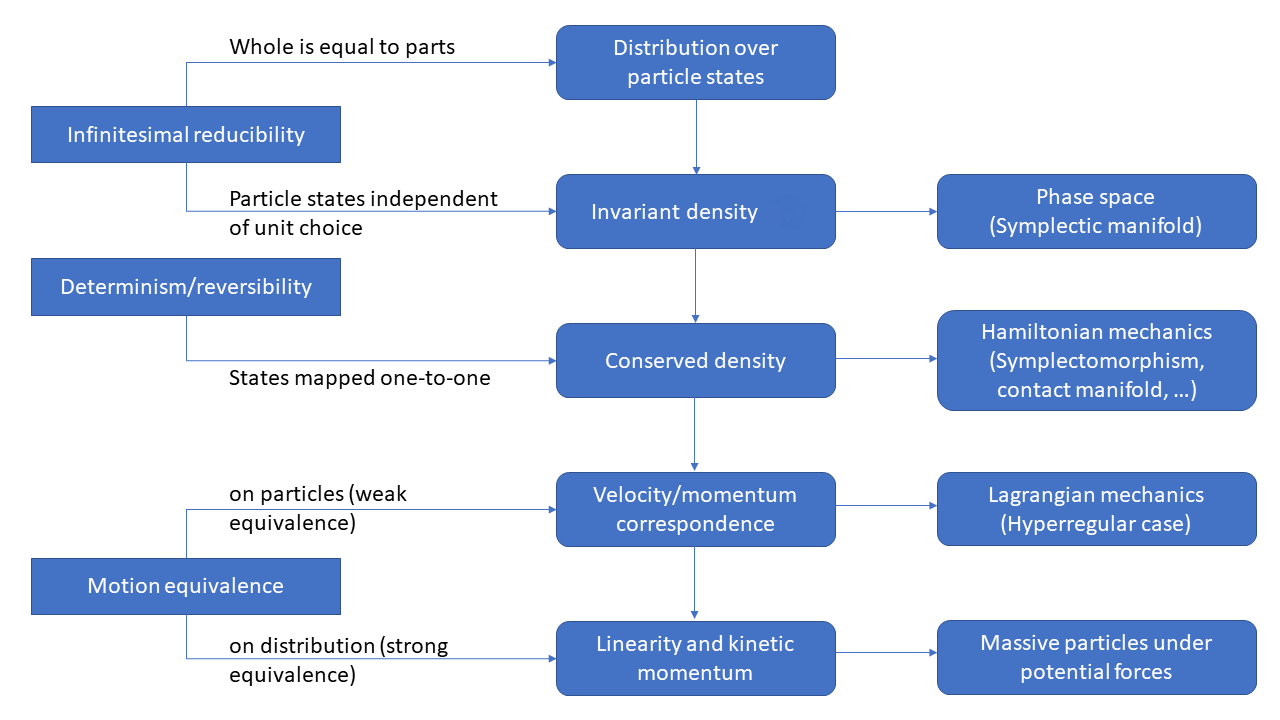
\includegraphics[width=\textwidth]{Diagram.png}
\caption{Physical conditions and corresponding properties and formalisms}
\label{diagram}
\end{figure}

%Like many arguments in physics, our derivation falls short of some norms on mathematical rigor. 
%optional to do: give a gloss on notion of regulative assumption (Kant and Peirce) 

\subsection{Infinitesimal reducibility}
\label{infinitesimal}

First, we will show that a classical phase space arises if a system satisfies the following physical condition 

\begin{quotation}
\bs \noindent
\textit{Infinitesimal reducibility}: the state of the system is reducible to the state of its infinitesimal parts. That is, specifying the state of the whole system is equivalent to specifying the state of its parts.
\es
\end{quotation}


\noindent
This assumption characterizes classical systems as those whose infinitesimal parts completely specify the state of the system. We define a \textit{classical particle} as one of these infinitesimal parts, namely the limit of recursive subdivision.\footnote{This definition of a classical particle differs from viewing point-particles as extensionless \parencites[]{Butterfieldpoints} or zero-dimensional \parencites[]{Wilson}.}
% % % For further discussion, see \textcites{shpmp}. [omit this for review].

Let $\mathcal{C}$ be the state space for the whole system, so that any $c \in \mathcal{C}$ represents a particular state of the whole system. Given infinitesimal reducibility, a classical system consists of a collection of classical particles. Let $\mathcal{S}$ be the state space for the particles, so that each point $s \in \mathcal{S}$ describes a possible state of a classical particle. Then for each system state $c \in \mathcal{C}$, there exists a unique distribution $\rho_c : \mathcal{S} \to \mathbb{R} $ that describes the state of $c$'s parts. That is, the state of the whole system is a distribution over its infinitesimal parts. This distribution describes the proportion of classical particles in any particular state from $\mathcal{S}$.
%ref 1: worth clarifying relationship between particle statespace S and system state space C. Is there an S_i for each i-th particle? And explain why we are not focusing on the statespace of the many particle system, e.g. a cartesian product of state spaces for each particle 

%If $\mathcal{S}$ is a discrete space with $U \subseteq \mathcal{S}$, we define $\mu(U) = \sum\limits_{s \in U} \rho_c(s)$ so that $\mu(\mathcal{S})$ gives us the size of the system and $\mu(U)/\mu(\mathcal{S})$ gives us the fraction of the particles that can be found in the region $U$.\footnote{The discrete case is far less interesting because discrete quantities cannot change continuously over time, meaning that they must be constant. We discuss this elsewhere.}
% % % For details see \textcites[]{AoPPhy1}. [omit this for review]}
% % XXX could try to find justification/derivation for the state space being a manifold in the Kevin Kelly book, or could cite the math paper with Greenfield; proposition 6.2. Try to include a better gloss/motivation for this claim (basic idea: if time is continuous, trajectories in state space must be continuous, local structure must be compatible). Curiel paper might also have a brief justification/motivation, if I recall


When the system is characterized by continuous quantities, $\mathcal{S}$ is a manifold. For $U \subseteq \mathcal{S}$, we define $\mu(U) := \int_U \rho_c(s) d\mathcal{S}$ to measure the number of particles in region $U$. \textit{State variables} $\xi^a$ are any set of quantities that fully identify states, so that $\xi$: $\mathcal{S} \to \mathbb{R}^n$ is an invertible function between each state and the numeric values of the variables.\footnote{In the language of manifolds, these $\xi^a$ are called ``coordinates'' and $\xi$ is a coordinate map. To avoid confusion, we will call the coordinates of the state space $\mathcal{S}$ ``state variables.'' As usual with coordinate charts, $\xi$ is properly defined on some $U \subseteq \mathcal{S}$, and $\xi^{-1}$ is defined on $\xi(U) \subseteq \mathbb{R}^n$. We will neglect these subtleties in what follows.} The map $\xi$ represents a state $s \in \mathcal{S}$ by a set of state variables $\xi^a \in \mathbb{R}^n$, such that $\xi (s) = \xi^a$. To represent the distribution $\rho_c$ in terms of state variables, we define a density $\rho_{c, \xi}$: $\mathbb{R}^n \to \mathbb{R}$ by $\rho_{c, \xi} \equiv (\rho_c \circ \xi^{-1})$. This density plays a crucial role throughout our argument. It allows us to compare and track the amount of matter in different possible states.

Since $\rho_c$: $\mathcal{S} \to \mathbb{R}$ is a function of the particle state $s$, we assume that its value is independent of the choice of state variables $\xi^a$ (i.e. the choice of state variable map $\xi$). If this assumption did not hold, then we could not model the system in the first place using state variables, and this would preclude many standard representational tools. Hence, the density $\rho_{c, \xi}$ must transform as a scalar under state variable changes.\footnote{For two state variable maps $\xi$ and $\hat{\xi}$, we have $\rho_c(s) = (\rho_c \circ \xi^{-1} \circ \xi)(s) = (\rho_c \circ \hat{\xi}^{-1} \circ \hat{\xi})(s)$, which entails that $\rho_c(s) = \rho_{c, \xi} (\xi^a) = \rho_{c, \hat{\xi}} (\hat{\xi}^b)$. Here, $\xi(s) \equiv \xi^a$ and $\hat{\xi}(s) \equiv \hat{\xi}^b$.} Likewise, we assume that the integral $\int_U \rho_c(s) d\mathcal{S} $ is independent of the choice of state variables, so that $\int_{\xi(U)} \rho_{c, \xi} (\xi^a) d \xi^a = \int_{\hat{\xi}(U)} \rho_{c, \hat{\xi}} (\hat{\xi}^b) d \hat{\xi}^b$.\footnote{Here, we assume that $\xi$ and $\hat{\xi}$ map the background measure on $\mathcal{S}$ to the standard Lebesgue measure on $\mathbb{R}^n$. In order to match integrands below, we also assume that $\xi$ and $\hat{\xi}$ agree on their orientation. These are regulative assumptions so that we can model the system using coordinates on $\mathbb{R}^n$. They amount to assuming that the particle state space $\mathcal{S}$ has a volume form.} Applying the change of variables formula, we know that $\int_{\hat{\xi}(U)} \rho_{c, \hat{\xi}} (\hat{\xi}^b) d \hat{\xi}^b= \int_{\xi(U)} \rho_{c, \hat{\xi}} (\hat{\xi}^b) \left|\frac{\partial \hat{\xi}^b}{\partial \xi^a} \right|  d \xi^a$.\footnote{The change of variables transformation from $\xi^a$ to $\hat{\xi}^b$ is given by $\phi \equiv \hat{\xi} \circ \xi^{-1}$: $\mathbb{R}^n \to \mathbb{R}^n $. For convenience, we denote $\rho_{c, \hat{\xi}} (\phi(\xi^a))$ by $\rho_{c, \hat{\xi}} (\hat{\xi}^b)$. Likewise, in the numerator of the Jacobian, we denote $\partial \phi$ by $\partial \hat{\xi}^b$, where $\hat{\xi}^b$ is here understood as a function of $\xi^a$.} Here, $ \left|\frac{\partial \hat{\xi}^b}{\partial \xi^a} \right|$ is the determinant of the Jacobian for this change of state variables. Matching integrands from the preceding two equations, we have $\rho_{c, \xi} (\xi^a) = \rho_{c, \hat{\xi}} (\hat{\xi}^b) \left|\frac{\partial \hat{\xi}^b}{\partial \xi^a} \right|$. From the scalar transformation property, $\rho_{c, \xi} (\xi^a) = \rho_{c, \hat{\xi}} (\hat{\xi}^b)$. Hence, we see that $\rho_{c, \hat{\xi}} (\hat{\xi}^b) =  \rho_{c, \hat{\xi}} (\hat{\xi}^b) \left|\frac{\partial \hat{\xi}^b}{\partial \xi^a} \right|$, entailing that the Jacobian determinant must equal one. By dimensional homogeneity, it must also be dimensionless. 

We will now show that in order for the density $\rho_{c, \xi}$ to have these transformation properties, the particle phase space $\mathcal{S}$ must be at least a symplectic manifold. In other words, given that i) we assume we can model a classical system by a density over its infinitesimal states and ii) these transformation properties are required for the density to play this role, it follows that the phase space must have a symplectic manifold structure. Our next assumption involves the relationship between state variables and measurement units. 
%Since these transformation properties are required to use a density to model a classical mechanical system, it follows that having the structure of a symplectic manifold is likewise required.  
%From the preceding two equations, we see that $\int_{\xi(U)} \rho_{c, \xi} (\xi^a) d \xi^a = \int_{\xi(U)} \rho_{c, \hat{\xi}} (\hat{\xi}^b) \left|\frac{\partial \hat{\xi}^b}{\partial \xi^a} \right|  d \xi^a$.
% $d \xi^a$ and $d \hat{\xi}^b$ are the

\subsubsection{The particle state space is even-dimensional}

We assume that a proper subset of the state variables suffices to define a unit system for all of the state variables. Again, this assumption is regulative in the sense that without it, we could not quantify properties of the system using measured values. Using this assumption, we will show that the state space $\mathcal{S}$ must be even-dimensional and hence a candidate for having symplectic structure. 

We define a \textit{unit variable} $q \in \xi^a$ as a particular state variable that defines a unit. For instance, $q$ might be position, defined in units of meters. Two unit variables are \textit{independent} if one unit variable can be changed without changing the other. For example, one can measure vertical position in meters while measuring horizontal position in miles.  The \textit{unit variables} $q^i$ are a privileged subset of the state variables that define the unit system. These $q^i$ determine the units not only for themselves, but for all other state variables. A \textit{change of units} is therefore a map $\hat{q}^j = \hat{q}^j(q^i)$ that defines new unit variables in terms of old unit variables. Since the unit variables define the units for all state variables, this change must induce a unique change of state variables $\hat{\xi}^b = \hat{\xi}^b(\xi^a)$ for all variables.
%to do: cite susan sterrett work on units as a `logical constraint'; , i.e. they fix the units for all state variables. 
%ref 2: mention that any transformation on the unit variables `is required to extend to a unique transformation of all the coordinates' 

Consider first the simplest case: suppose that a single unit variable $q $ suffices to define the unit system for the particle state space. Then, the state variables are a set $\xi^a = \{ q, k^\alpha \}$, where \textit{prima facie} the index $\alpha$ could be any non-negative integer. We will show that, in fact, there must be exactly one $k^\alpha$ variable, conjugate to the single $q$ variable. 

As a scalar, the units of the density $\rho_{c, \xi}$ are invariant under unit changes of the state variables. Suppose we change units by transforming $q$ to a new unit variable $\hat{q}=\hat{q}(q)$. Call the new state variables $\hat{\xi}^b = \{ \hat{q}, \hat{k}^\beta\}$. As shown above, the Jacobian determinant $\left|\frac{\partial \hat{\xi}^b}{\partial \xi^a} \right|$ must equal one. Assume for contradiction that there is only one state variable, so that there are no $k^\alpha$ variables. Then we would have $\left|\frac{\partial \hat{\xi}^b}{\partial \xi^a} \right| = \left|\frac{\partial \hat q}{\partial q} \right| = 1$. But this would mean the unit change cannot be arbitrary. Therefore we must have two or more state variables, requiring at least one $k^\alpha$ variable. 

Next, we show that in fact there must be exactly one $k$ variable, conjugate to the single $q$ variable. Using the fact that the Jacobian determinant equals one, we determine how the state variables $k^\alpha$ must change in order to compensate the change from $q$ to $\hat q$. Since $\hat{q}$ depends only on $q$, $\frac{\partial \hat{q}}{\partial k^\alpha} = 0$. Hence, the Jacobian is a lower triangular block matrix: 
\begin{equation}
%\begin{aligned}
|J| = \left|\frac{\partial \hat{\xi}^b}{\partial \xi^a} \right| = \begin{vmatrix}
\frac{\partial \hat{q}}{\partial q} & \frac{\partial \hat{q}}{\partial k^\alpha} \\
\frac{\partial \hat{k}^\beta}{\partial q} & \frac{\partial \hat{k}^\beta}{\partial  k^\alpha} 
\end{vmatrix} = \begin{vmatrix}
\frac{\partial \hat{q}}{\partial q} & 0 \\
\frac{\partial \hat{k}^\beta}{\partial q} & \frac{\partial \hat{k}^\beta}{\partial  k^\alpha}
\end{vmatrix}
%\end{aligned}
\end{equation}

\noindent
The determinant of a triangular block matrix equals the product of determinants of the block matrices along the diagonal: $ \left|\frac{\partial \hat{\xi}^b}{\partial \xi^a} \right| =  \left|\frac{\partial \hat{q}}{\partial q}\right| \left|\frac{\partial \hat{k}^\beta}{\partial k^\alpha}\right|$. For the Jacobian determinant to equal one, we must therefore have  $\left|\frac{\partial \hat{k}^\beta}{\partial k^\alpha} \right| =   \left|\frac{\partial \hat{q}}{\partial q}\right|^{-1}$. Since $\hat q$ is a function only of $q$, $\frac{\partial \hat{q}}{\partial q}$ is a total derivative, so we obtain the inverse by swapping the numerator and denominator. Hence, we see that $\left|\frac{\partial \hat{k}^\beta}{\partial k^\alpha} \right| = \left|\frac{\partial q}{\partial \hat q} \right|$. 
%  $\left|\frac{\partial \hat{q}}{\partial q}\right|^{-1} = \left|\frac{\partial q}{\partial \hat q} \right|$. 

This equation provides only a single constraint, placed on the determinant of the transformation from $k^\alpha$ to $\hat{k}^\beta$. Hence, if there were three or more $\xi^a$ variables, this constraint would be insufficient to recover the transformation of the $k^\alpha$ uniquely. In this case, $\hat q$  would not fully define the units for all other state variables, contrary to assumption. Consequently, there must be exactly two state variables: $q$ and a single $k$. So in the case of a single $q$ variable, defining an invariant density $\rho_{c, \xi}$ requires a two-dimensional manifold.

We extend this construction to the general case with multiple unit variables $q^i$. Recall that two unit-variables are independent if changing the units for one does not change the units for the other. Suppose our particle state space $\mathcal{S}$ is such that its units are fully defined by $n$ independent unit-variables $q^i$. If we change the first unit-variable $q^1$ without changing the others, then the variable $k_1$ must change as before, so that the density remains invariant. Likewise, transforming the second unit-variable $q^2$ in the same way (while fixing $k_1$) requires a corresponding $k_2$. Continuing, we find that $\mathcal{S}$ is $2n$-dimensional, with state variables $\xi^a = \{ q^i, k_i \}$. We define an \textit{independent degree of freedom} as the space charted by a pair of such variables. Each independent degree of freedom thereby defines a two-dimensional surface in phase space. These play a crucial role in showing that $\mathcal{S}$ must have a non-degenerate, closed two-form $\omega$, i.e. a symplectic form. 

\subsubsection{The particle state space has a symplectic form}

We now show that $\mathcal{S}$ must have a well-defined two-form $\omega$. Recall that a density is defined in terms of an amount per unit volume. Representing the system state $c$ in terms of its infinitesimal parts requires that the density $\rho_{c, \xi} $ is defined on infinitesimal volumes $d \mathcal{S}$ of the phase space. Since each independent degree of freedom comprises a pair of state variables, each infinitesimal volume decomposes into independent infinitesimal areas. To define the density $\rho_{c, \xi} $, we must be able to measure each of these independent infinitesimal areas. This is precisely the role performed by a two-form $\omega$, which assigns an infinitesimal area to each infinitesimal surface. We can then define integrals of the form $\int_{\Sigma} \rho_c \omega(d\Sigma)$, for $\Sigma \subset \mathcal{S}$ (i.e. the fraction of the system whose parts are in the region $\Sigma$ of state space $\mathcal{S}$). Because the degrees of freedom are independent, the total number of states in a volume is the product of the possible configurations of each degree of freedom. This means that the volume form is given by $\omega^n$. 

Since each volume of phase space contains some possible states, the volume form cannot be degenerate. If the volume form were degenerate, then there would be a ``volume'' in state space that did not contain states. But then this region of state space could not be a volume. Since the volume form $\omega^n$ is non-degenerate, the two-form $\omega$ must also be non-degenerate. Otherwise, there would be infinitesimal surfaces in phase space assigned zero area, i.e. there would be states of phase space that $\omega$ does not count. But, $\omega$ must count all possible states in order for the density $\rho_{c, \xi} $ to be well-defined.


%on needing a two-form to measure areas, could possibly cite Strang 1993, ch. 5 or Mac Lane & Birkhoff (1999, Theorem IX.2.2). 
%note: an infinitesimal area counts the number of possible states in a region of phase space, as given by the two state variables that compose the degree of freedom

Next, we show that $\omega$ must be closed, using the fact that the degrees of freedom are independent. If we translate a surface along an independent degree of freedom, this does not change the area of the surface, meaning that the number of states on that surface is invariant. We can therefore construct a parallelepiped $P$, whose opposite sides have equal areas. Integrating $\omega$ over the closed surface $\partial P$ of this parallelepiped, opposite sides provide equal and opposite contributions. Hence, the integral over this closed surface must equal zero: $\int_{\partial P} \omega =0$. By Stokes' theorem, the integral of $d \omega$ over this volume $P$ must equal zero as well: $\int_P d \omega = \int_{\partial P} \omega =0$. Since, we can approximate any volume $V$ by such parallelepipeds, $\int_V d \omega = 0$ for arbitrary $V$. Hence, the integrand $d \omega$ must vanish, entailing that $\omega$ is closed. So $\mathcal{S}$ must come equipped with a two-form $\omega$ that is closed and not degenerate, and therefore $\mathcal{S}$ is a symplectic manifold.

Moreover, the units we choose for $\omega$ are the units we choose to count states over an independent degree of freedom. This agrees with the practice in statistical mechanics. When normalized, the density $\rho_{c, \xi}$ is given in terms of the inverse of the units for $\omega$. In accordance with the standard conventions in quantum mechanics and statistical mechanics, the $k_i$ are given in terms of inverse units of the respective $q^i$, such that $dq^i \wedge dk_i$ is a pure number. We then use $\hbar$ to define the units for state counting and therefore set $\omega = \hbar dq^i \wedge dk_i = dq^i \wedge dp_i$ where $p_i = \hbar k_i$.

We can thereby understand canonical coordinates as a set of state variables that express the density in the correct units. A canonical transformation is one that preserves the unit and the numerical value of the density. A change of unit is a special type of canonical transformation: one where we have an arbitrary change in the unit variables and an induced (covariant) change in the conjugate variables.
 
 
In sum, under the infinitesimal reducibility assumption, a state $c$ of the system is represented by a coordinate-invariant density over the state space $\mathcal{S}$ of its infinitesimal parts. We have shown that the state space of the particles must be a symplectic manifold. Additionally, any symplectic manifold structure supports the definition of coordinate-invariant densities: any scalar function can be integrated using the symplectic form in a coordinate-invariant way. Therefore symplectic structure is exactly the structure needed to define an invariant density. 

%Section~\ref{density} describes further interpretive consequences of this connection between invariant densities and symplectic structure.


\subsection{Deterministic and reversible evolution}
\label{deterministic}

Next, we focus on those classical systems that are deterministic and reversible. This amounts to satisfying the following joint condition:

\begin{quotation}
\bs
\noindent
\textit{Deterministic and reversible evolution}: given the present state of the system, all future (determinism) and past (reversibility) states are uniquely identified. \es
\end{quotation}

\noindent In our case, this applies to both the state of the whole system and the state of its parts. 

First, we will show that deterministic and reversible evolution entails that the density $\rho_{c, \xi}$ is constant in time. We consider a particle state $s_0$ at time $t_0$. Given deterministic and reversible evolution, there exists a unique evolution $\lambda: \mathbb{R} \to \mathcal{S}$ such that $\lambda(t_0) = s_0$. Hence, the initial state $s_0$ at time $t_0$ uniquely identifies the state of this particle at all times. Let $\rho(s, t)$ be the density associated to a state $s$ at a time $t$.\footnote{For convenience, we sometimes drop the composite state $c$ and coordinate-choice $\xi$ indices from the invariant density $\rho_{c, \xi} (\xi^a)$. We reserve the word ``distribution'' for the coordinate-free distribution $\rho_c (s)$. } Then  $\rho(\lambda(t_0), t_0)$ represents the part of the composite system in particle state $s$ at that time. Likewise, for $t_1 > t_0$,  $\rho(\lambda(t_1), t_1)$ represents the part of the system associated to the evolved state at this future time. Given deterministic and reversible evolution, all particles that start in a given initial state must end up in the same final state, and vice-versa. Hence, $\rho(\lambda(t_0), t_0) = \rho(\lambda(t_1), t_1)$ for all $t_0,\, t_1$. In other words, the density remains the same throughout the evolution.
%Let $\lambda: \mathbb{R} \to \mathcal{S}$ be the evolution over time of the state of a particle. 


Second, we show that the two-form $\omega$ is invariant under this evolution, and hence that the system follows Hamiltonian evolution. Consider a surface $\Sigma_0 \subset \mathcal{S}$ of particle states at some time $t_0$. If two-dimensional, this surface defines an independent degree of freedom. The integral $\int_{\Sigma_0} \rho_c (s, t_0) \omega(d\Sigma_0)$ represents the fraction of the system in states defined on $\Sigma_0$. Since each particle state evolves by $\lambda$, $\Sigma_0$ evolves to a surface $\Sigma_1$ at time $t_1$. This leads to a corresponding $\int_{\Sigma_1} \rho_c (s, t_1) \omega(d\Sigma_1)$, representing the fraction of the system on this evolved surface. Since the evolution is deterministic and reversible, all and only the particle states that began on surface  $\Sigma_0$ evolve to $\Sigma_1$. Consequently, the fraction of the system on these two surfaces at these two times must be the same: $\int_{\Sigma_0} \rho_c (s, t_0) \omega(d\Sigma_0) = \int_{\Sigma_1} \rho_c (s, t_1) \omega(d\Sigma_1)$. Since the density is constant, we know that $\rho_c (s, t_0) = \rho_c (s, t_1)$. Hence, the two-form $\omega$ must remain the same. That is, the areas in phase space must be mapped to areas of equal size, and independent degrees of freedom must be mapped to independent degrees of freedom (otherwise, volumes would not be mapped to equal volumes, violating determinism). The evolution is therefore a symplectomorphism and hence corresponds to a Hamiltonian evolution. 
%Now consider the integral $\int_{\Sigma} \rho_c \omega(d\Sigma)$. Mapping the region $\Sigma$ to a new region, the fraction of the system found in both the old and new regions must be the same. Since both the integral and $\rho_c$ must remain constant during the evolution, the two-form $\omega$ must also remain the same. 

Intuitively, our argument is the inverse of Liouville's theorem: instead of positing Hamiltonian evolution and finding conservation of areas and volumes, deterministic and reversible evolution imposes the conservation of areas and volumes (i.e. sets of states are mapped to sets of states of equal size). This leads to Hamiltonian evolution. In summary, we have shown that any system that satisfies the conditions of both infinitesimal reducibility and deterministic/reversible evolution is a classical Hamiltonian system.
% [(ref 1): expand on how our argument relates to standard proofs of Liouville's theorem. Is it fair to say that we are privileging Hamiltonian mechanics because it forms the basis for a proof of Liouville's theorem?]


\subsection{Motion equivalence}
\label{motion}

Having recovered classical Hamiltonian mechanics, the laws of evolution are further restricted when the following condition holds:


\begin{quotation}
\bs \noindent
\textit{Motion equivalence}: the motion of the system (i.e. trajectories in physical space) suffices to recover its dynamics (i.e. evolutions in state space) and vice-versa.\footnote{ \textcites[218]{Abraham}, Theorem 3.6.2 shows that in the hyper-regular domain, Lagrangian and Hamiltonian mechanics describe the same evolution of particle positions over time; see \textcites[1180-1181]{Barrett2} for discussion. Motion equivalence can be understood as the converse of this theorem: assuming that Lagrangian and Hamiltonian mechanics agree on particle evolutions, we derive that the Legendre transformation is well-defined in the hyper-regular domain.} \es
\end{quotation}


\noindent If we focus on the parts of the system, this means that for every evolution in phase space there should be one and only one trajectory in physical space. 

Note that each space variable $x^i$ is a unit-variable, i.e. a state variable that defines a unit. In fact, the trajectories can be fully described only by these unit-variables. For, to specify a trajectory, we need epistemic access to a unit system, where the number of independent units is determined by the dimensionality of physical space. It follows that (i) $x^i = q^i$, (ii) each $q^i$ is paired with a conjugate $p_i$, and (iii) each state $\{q^i, p_i\}$ corresponds to one and only one trajectory in physical space. 

At each point $x^i$, then, there must be infinitely many trajectories, one for each possible combination of $\{p_i\}$. Since these trajectories are differentiable in $x^i$, we can define a velocity $v^i = d_t x^i$. If the equations of motion contained the velocity as a function of only the unit-variables (i.e. $v^i=v^i(q^i)$), then motion equivalence would fail. For if both $x^i$ and $v^i$ were functions of only $q^i$, this relationship would not be invertible due to dimensional considerations (a surjection from an $n$-dimensional manifold to a $2n$-dimensional manifold cannot be invertible). Hence, we must have $v^i=v^i(q^j, p_k)$, so that knowledge of the state in phase space suffices for knowledge of the trajectory. If motion equivalence holds, then this relationship must be invertible, meaning that knowledge of the trajectory suffices for knowledge of the phase space state. For systems that satisfy the motion equivalence condition, the following relationships thus hold at any given time:
\begin{equation}\label{weak_equivalence}
\begin{aligned}
x^i &= q^i \\
v^i &= d_t x^i = v^i(q^j, p_k)
\end{aligned}
\end{equation}

In this case---which we call \textit{weak equivalence}---$v^i(q^j, p_k)$ is invertible at every $q^j$. Therefore, for fixed $q$, the Jacobian matrix  $\frac{\partial v^i}{\partial p_k}$ must be invertible. Let $H$ denote the Hamiltonian. By Hamilton's equations, $v^i = d_t q^i = \frac{\partial H}{\partial p_i}$, so the Hessian $\frac{\partial^2 H}{\partial p_k \partial p_i} = \frac{\partial}{\partial p_k} (\frac{\partial H}{\partial p_i})$ equals the Jacobian $\frac{\partial v^i}{\partial p_k}$. Since the Jacobian is invertible, the Hessian must be non-zero everywhere, and therefore it must have the same sign everywhere---which we take to be positive. Weak equivalence allows us to express particle states in terms of either position/momentum or position/velocity variables. These are exactly the cases where a Lagrangian can be constructed, and where the Lagrangian leads to a unique solution (via the stationary action principle). Hence, weak equivalence suffices for the existence of a hyper-regular Lagrangian.\footnote{Weak equivalence corresponds to a general treatment of Lagrangian mechanics that does not presuppose Riemannian geometry. As we discuss in Section~\ref{Curiel}, Equation~\ref{weak_equivalence} corresponds to the kinematical constraints central to Curiel's \parencites*[]{Curiel} argument for privileging Lagrangian mechanics.}

Whereas weak equivalence involves motion equivalence at the level of particle states, \textit{full equivalence} extends this to the entire distribution, i.e. the composite state of the system. Full equivalence holds when we can express the distribution---represented by the density---in terms of position and velocity variables. Formally, this requires that $\rho(q^i, p_j) = |J| \rho(x^i, v^j) = \left|\frac{\partial v^i}{\partial p_j}\right| \rho(x^i, v^j)$ since
\begin{equation}
\begin{aligned}
|J| &= \begin{vmatrix}
\frac{\partial x^i}{\partial q^j} & \frac{\partial x^i}{\partial p_j} \\
\frac{\partial v^i}{\partial q^j} & \frac{\partial v^i}{\partial p_j}
\end{vmatrix}
= \begin{vmatrix}
\delta^i_j & 0 \\
\frac{\partial v^i}{\partial q^j} & \frac{\partial v^i}{\partial p_j}
\end{vmatrix} \\
&= \left|\delta^i_j\right| \left|\frac{\partial v^i}{\partial p_j}\right| 
= \left|\frac{\partial v^i}{\partial p_j}\right|.
\end{aligned}
\end{equation}
Note that while the value given by $\rho(q^i, p_j)$ is invariant under unit changes, the value given by $\rho(x^i, v^j)$ depends on the choice of units through $\left|\frac{\partial v^i}{\partial p_j}\right|$. If $x^i$ truly sets the unit system by itself, then $\left|\frac{\partial v^i}{\partial p_j}\right|$ must be a function of position only, since the position variables define the units. Similar considerations hold for marginal distributions (i.e. distributions on a subset of the unit variables), entailing that all components of $\frac{\partial v^i}{\partial p_j}$ must be a function of position only. We set:
%\footnote{In Section~\ref{dependence}, we will see that $g^{ij}$ corresponds to the Riemannian metric, since $\partial v^i/\partial p_j$ is a function only of position.}
\begin{equation}
\begin{aligned}
\frac{\partial v^i}{\partial p_j} = \frac{1}{m} g^{ij} \\
\frac{\partial p_j}{\partial v^i} = m g_{ji}
\end{aligned}
\end{equation}
where $m$ is the unit conversion constant between velocity and conjugate momentum, while $g_{ij}$ represents the linear dependency of the velocity on the momentum. 

If we integrate, we have:
\begin{equation} \label{linear_relationship}
\begin{aligned}
v^i = \frac{1}{m} g^{ij}(p_j - A_j) \\
p_j = m g_{ji} v^i + A_j
\end{aligned}
\end{equation}
where $A_j$ are arbitrary functions. We recognize $m g_{ji} v^i$ as kinetic momentum. Note that:
\begin{equation}
v^i = d_t q^i = \frac{\partial H }{\partial p_i} = \frac{1}{m} g^{ij}(p_j - A_j) 
\end{equation}
We integrate yet again and find:
\begin{equation} \label{massive_Hamiltonian}
H = \frac{1}{2m} (p_i - A_i) g^{ij}(p_j - A_j) + V 
\end{equation}
where V is another arbitrary function. We recognize this as the Hamiltonian for massive particles under potential forces, relevant for classical electrodynamics and Newtonian gravitation. For example, $A$ can play the role of the magnetic vector potential, with $V$ playing the role of the electric potential. Whereas Curiel \parencites*[]{Curiel} argues that this Hamiltonian requires the imposition of \textit{ad hoc} conditions, we take ourselves to have given an eminently natural construction of it. We return to this point in Section~\ref{Curiel}, using it to defuse Curiel's argument for the primacy of Lagrangian mechanics.

This completes our primary argument for privileging Hamiltonian mechanics over Lagrangian mechanics. We have seen that Lagrangian systems are a proper subset of Hamiltonian systems, specifically those Hamiltonian systems that also satisfy the motion equivalence condition. In the next section, we provide a geometric interpretation of the principle of stationary action within Hamiltonian mechanics. Our construction makes manifest the gauge-dependency of the Lagrangian, providing a further reason to privilege the Hamiltonian. Finally, we respond to Curiel's arguments against the fundamentality of Hamiltonian mechanics.
% In the remainder of this essay, we provide further reasons for privileging Hamiltonian mechanics. The next section describes how Hamiltonian mechanics provides the natural setting for the invariant density, which characterizes how a classical object's parts are distributed. The invariant phase space density is more fundamental than the state variables, since conjugate momentum is a gauge-dependent quantity. 



\section{Interpreting Lagrangian mechanics}
\label{Lagrangian}

By viewing classical systems through their invariant phase space density, we gain new insights into Lagrangian mechanics. Section~\ref{action} uses the invariant phase space density to give a geometric interpretation the action principle. We show that this principle holds even when the action is not defined as a function of position and velocity, since it can always be expressed as a function of position and conjugate momentum. Our construction makes the gauge-dependence of the Lagrangian manifest. Section~\ref{Curiel} considers Curiel's \parencites*[]{Curiel} argument for privileging Lagrangian mechanics, which he alleges encodes the necessary and sufficient structure for capturing the physically significant kinematical constraints of classical systems. This raises a number of objections to our own position, which we rebut. In short, we  argue that we have given a natural construction of Hamiltonian mechanics.
%In short, we argue that we have given an eminently natural construction of Lagrangian mechanics, viewed as a special case of Hamiltonian mechanics. Moreover, our argument shows that Lagrangian mechanics is in some sense less natural than Hamiltonian mechanics because the former is contingent on having a bijection between velocity and conjugate momentum. 


\subsection{A geometric interpretation of the action principle}
\label{action}

% Somewhere below, emphasize that you have a unique trajectory only if the action is a minimum or maximum (if it is just stationary but not a minimum or maximum, then you do not have a unique trajectory)

Hamilton's principle of stationary action serves as a foundational principle for Lagrangian mechanics. According to this principle, infinitesimal variations of the action $ \mathscr{A}$ along the system's trajectory $\gamma $ equal zero: $\delta  \mathscr{A}[\gamma] = 0 $. Although central to Lagrangian mechanics, we can actually derive the stationary action principle using Hamiltonian mechanics. Our derivation simply assumes that the system's trajectory follows a deterministic and reversible evolution. We present the derivation for the one-dimensional case---where it is most easily visualized---but it can be generalized using differential geometry.\footnote{For a related argument, see \textcites[236--37, 243--45]{Arnold}.}

The derivation uses the extended phase space $(q, p, t)$, i.e. the standard phase space extended by the time variable. Knowing that the system is deterministic and reversible, it follows from Section~\ref{deterministic} that the density of states is invariant. This means that possible trajectories of the system in the extended phase space are never pushed toward each other or pulled apart over time. In other words, the flux of trajectories through any closed surface in the extended phase space is always zero. Formally, the vector field $\vec{S} := (\frac{d q }{d t }, \frac{d p }{d t }, \frac{d t }{d t })$ represents the displacement of states along the trajectories. This field is divergenceless, $\nabla \cdot \vector{S} = 0$, because for any region $U$, the same number of states will enter the region as exit. Moreover, note that the displacement vector $\vec{S}$ is tangent to the trajectory $\gamma [q, p, t] (t)$ in extended phase space, where the variable $t$ functions as both a coordinate and the evolution parameter.

Since $\vector{S}$ is divergenceless, there exists another vector field $-\vector{\theta}$ such that $\vector{S} = curl(-\vector{\theta} )$.\footnote{For reasons that will become clear, we choose $-\vector{\theta}$ rather than $\vector{\theta}$.} As a vector field in the extended phase space, $\vector{\theta}$ can be written in terms of its components $\vector{\theta} = (\theta_q, \theta_p, \theta_t) $. Since the curl of the gradient of a scalar function is always zero, the displacement vector $\vector{S}$ is invariant under the gauge transformation $\vector{\theta'} =\vector{\theta} + grad(f)$, where $f$ is an arbitrary scalar function. Hence, we can choose $f$ such that $\partial f/ \partial p = -\theta_p $. Without loss of generality, we can thereby redefine $\vector{\theta}$ as $(\theta_q, 0, \theta_t) $.

Treating time $t$ as both a coordinate and the evolution parameter, the time component of the displacement $S_t = dt/ dt = 1$.\footnote{In the expression ``$dt/dt$,'' the time variable in the numerator functions as a coordinate, while the time variable in the denominator functions as a parameter. We could instead use a parameter $\tau$, and the derivation would remain valid.} This places another constraint on $\vector{\theta} $, since $\vector{S} = -curl(\vector{\theta}) $. In components, this means that $S_t = - (\frac{\partial}{\partial q} \cdot \theta_p - \frac{\partial}{\partial p} \cdot \theta_q) = - (\frac{\partial}{\partial q} \cdot 0 - \frac{\partial}{\partial p} \cdot \theta_q) = \frac{\partial \theta_q}{\partial p}$. Hence, $S_t = 1$ entails that $\frac{\partial \theta_q}{\partial p} = 1$. Integrating this expression, we find that $\theta_q = p$ up to addition by an arbitrary constant function $g(q)$. Again using the gauge freedom of $\vector{S}$, we can set $g(q)=0$, so that $\theta_q = p$. Thus far, we have shown that $\vector{\theta} = (p, 0,\theta_t) $.

Next, we introduce a function $H$ and let $ \theta_t \equiv -H$. Hence, we write $-\vector{\theta} = (-p, 0, H) $ as the vector potential for the displacement vector $\vector{S} $. By matching components of $\vector{S}$ and $-curl(\vector{\theta})$, we show that $H$ is the Hamiltonian for the system. First, by definition, $S_q \equiv \frac{dq}{dt} $ and $S_p \equiv  \frac{dp}{dt} $. Secondly, since $\vector{S} = -curl(\vector{\theta}) $, we calculate that $S_q = -\frac{\partial \theta_t}{\partial p} = \frac{\partial H}{\partial p}$ and $S_p = \frac{\partial \theta_t}{\partial q}=-\frac{\partial H}{\partial q}$. Matching terms, we see that $\frac{\partial H}{\partial p} =\frac{dq}{dt} $ and $-\frac{\partial H}{\partial q} =\frac{dp}{dt}$. These simply are Hamilton's equations, which justifies interpreting $H$ as the Hamiltonian.

At this point, we return to the action $ \mathscr{A}$. If the motion equivalence condition holds, then $ \mathscr{A}$ is defined as the integral of the Lagrangian over a trajectory beginning at time $t_0$ and ending at time $t_1$: $\integral^{t_1}_{t_0} L (q, \dot{q}, t) dt$. If motion equivalence does not hold, we can define the action more generally over the function $L_p \equiv p \dot{q} - H(q, p, t)$, considering paths in the extended phase space. By deriving the stationary action principle in this more general setting, we simultaneously derive its usual version within Lagrangian mechanics. We have then that $ \mathscr{A}[\gamma] = \integral^{t_1}_{t_0} L_p (q, p, t) dt = \integral^{t_1}_{t_0} [p \frac{dq}{dt} - H(q, p, t) ]dt$, where $\gamma$ is an actual trajectory followed by the system. Multiplying the Hamiltonian by $dt/dt = 1$ and adding a vanishing $0 \cdot \frac{dp}{dt}$, we obtain $ \mathscr{A}[\gamma] = \integral^{t_1}_{t_0} [p \frac{dq}{dt} + 0 \cdot \frac{dp}{dt} - H(q, p, t) \frac{dt}{dt} ]dt$. We notice that the integrand simply equals the inner product of $\vector{\theta}$ with $\vector{S} $, entailing that $L_p =\vector{\theta} \cdot \vector{S} $. Consequently, the action $ \mathscr{A} [\gamma] = \integral^{t_1}_{t_0} \vector{\theta} \cdot \vector{S}  dt$. Note that $\vector{S}  dt = (\frac{d q }{d t } dt, \frac{d p }{d t } dt, \frac{d t }{d t }dt ) = (dq, dp, dt) = d\vector{\gamma}$ represents the infinitesimal displacement along the trajectory. Therefore, the action equals the line integral of $\vector{\theta}$ along the trajectory $\gamma $: $ \mathscr{A} [\gamma] =\integral_{\gamma} \vector{\theta} \cdot d\vector{\gamma}$. To derive Hamilton's principle of stationary action, it suffices to show that $\delta \mathscr{A} [\gamma] =\delta \integral_{\gamma} \vector{\theta} \cdot d\vector{\gamma} = 0$. 

By definition, a variation over the integral $\integral_{\gamma} \vector{\theta} \cdot d\vector{\gamma}$ consists in taking the difference between the integrand and a corresponding integral over a nearby trajectory $\gamma'$: $\delta \integral_{\gamma} \vector{\theta} \cdot d\vector{\gamma} = \integral_{\gamma} \vector{\theta} \cdot d\vector{\gamma} - \integral_{\gamma'} \vector{\theta} \cdot d\vector{\gamma'}$ . Since the trajectories $\gamma$ and $\gamma'$ have the same endpoints, they define a closed-curve $C$, enclosing a region $\Sigma $. Hence, by Stokes' theorem $\delta \integral_{\gamma} \vector{\theta} \cdot d\vector{\gamma} = \oint_{C} \vector{\theta}  \cdot \vector{dC} = \iint_{\Sigma} curl(\vector{\theta}) \cdot \diff \vector{\Sigma}$ . Recalling that i) the $curl(\vector{\theta})$ equals the negative of the displacement vector $\vector{S}$, and ii)  $\vector{S}$ is tangent to the trajectory $\gamma $, we see that $curl(\vector{\theta})$ is tangent to the surface $\Sigma $.\footnote{Since $\vector{S}$ is tangent to $\gamma $, and $\gamma'$ defines an infinitesimal variation, it follows that $\vector{S}$ is tangent to the entire surface $\Sigma $.} Hence, the surface integral must vanish, showing that $\delta \integral_{\gamma} \vector{\theta} \cdot d\vector{\gamma}$ does indeed equal zero. This establishes a more general version of Hamilton's principle of stationary action, which we have derived simply by assuming that the displacement vector is divergenceless. In the special case that motion equivalence holds, the Legendre transformation is well-defined and $L_p = p \dot{q} - H(q, p, t)$ equals the usual Lagrangian $L(q, \dot{q}, t)$, thereby recovering the principle of stationary action for Lagrangian mechanics. 

As a corollary, this construction shows that the Lagrangian $L =\vector{\theta} \cdot \vector{S} $ is manifestly gauge-dependent. The vector potential $\vector{\theta}$ is gauge-dependent because we can transform it by adding the gradient of an arbitrary scalar function. The displacement vector $\vector{S} = curl(-\vector{\theta})$ is invariant under this gauge transformation. Hence, $L$ must be gauge-dependent, which complicates the physical interpretation of any particular Lagrangian. In contrast, the Hamiltonian is defined up to a constant, endowing it with greater physical significance.


\subsection{Curiel's privileging of Lagrangian mechanics}
\label{Curiel}

% Helpful summary of Curiel's position: ``Hamiltonian mechanics does not respect the kinematical constraints intrinsic to abstract classical systems'' while ``Lagrangian mechanics always respect[s] the kinematical constraints of abstract classical systems'' \parencites*[304]{Curiel}.

Curiel argues that Lagrangian mechanics represents classical mechanical systems in a \textit{natural} manner whereas Hamiltonian mechanics involves an essentially artificial construction \parencites*[270]{Curiel}.\footnote{Curiel characterizes ``natural'' in terms of natural coordinate systems, defined using the almost-tangent structure of the tangent bundle \parencites*[290-291]{Curiel}. He also uses the almost-tangent structure to give a general characterization of what he takes to be the fundamental kinematical constraints.} According to Curiel, all physically-meaningful classical systems satisfy a certain set of kinematic constraints. In the simplest case, these constraints characterize velocity as the first temporal derivative of position: $v^i = d_t x^i = v^i(q^j, p_k)$ (Equation~\ref{weak_equivalence}).\footnote{Curiel treats this constraint as ``kinematical'' in the sense that it must hold independently of the interactions between a system and its environment. He interprets it as a substantive physical condition, rather than an analytic truth \parencites*[282]{Curiel}.} Curiel argues that Lagrangian mechanics encodes the necessary and sufficient conditions for a system to satisfy these kinematic constraints, both within and outside the hyper-regular domain \parencites*[307--308, 311]{Curiel}. In contrast, Hamiltonian mechanics does not automatically encode these constraints. Since Curiel views these constraints as an essential feature of physically-meaningful classical systems, he argues that Lagrangian mechanics picks out the proper class of classical systems. 

Imposing these kinematic constraints within the Hamiltonian formalism requires focusing on a proper subset of all possible Hamiltonians. Within this subset, conjugate momentum is a linear function of velocity: $p_i = \lambda^j_i \dot{q}_j $ \parencites*[304]{Curiel}. This relationship between momentum and velocity entails that the Hamiltonian takes the following quadratic form---where the functions $U$ and $\alpha^{m n}$ are arbitrary functions of the generalized position coordinates $q_i$:
\begin{equation} \label{6.2}
H =\alpha^{m n} p_m p_n + U (q_j) 
\end{equation}
Curiel contends that this form is the ``necessary and sufficient condition [a Hamiltonian must have] for it to model an abstract classical system'' \parencites*[305]{Curiel}. Since many possible Hamiltonians do not take this form,\footnote{As an example, Curiel considers the Hamiltonian $H = \frac{1}{2} p_i p^i + \sum_j p_j$  \parencites*[305]{Curiel}.} Curiel believes we must artificially restrict Hamiltonian mechanics to those systems that satisfy Equation~\ref{6.2}.

To rebut Curiel's argument, it suffices to provide a natural interpretation of (\ref{6.2}). We have in fact already provided one in Section~\ref{motion}. There, we saw how both the linear relationship between momentum and velocity and the quadratic form (\ref{6.2}) follow from imposing the motion equivalence condition. In Equation~\ref{linear_relationship}, we recovered the linear relationship between conjugate momentum and velocity, up to the addition of an arbitrary function. Just as Curiel does, we then used this relationship to derive a quadratic form for the Hamiltonian (Equation~\ref{massive_Hamiltonian}). Imposing motion equivalence thereby allows us to interpret this quadratic form as the Hamiltonian for massive particles under potential forces. It is not an \textit{ad hoc} condition imposed on Hamiltonian systems. Instead, it arises in all contexts where motion equivalence holds, i.e. where the trajectory of the system in physical space is necessary and sufficient for its evolution in state space. Thus, we take ourselves to have responded to Curiel's main criticism of Hamiltonian mechanics, namely that it must impose \textit{ad hoc} the condition (\ref{6.2}). 
% Note that our equation 2 (\ref{weak_equivalence}) is a special case (or less mathematically sophisticated formulation) of Curiel's kinematic conditions, i.e. his equation 4.3 in terms of the almost-tangent structure. Our equation 2b matches Curiel's equations 3.1a and 3.2b, in the case of free and non-free Newtonian particles, respectively.

Furthermore, Curiel's definition of ``classical systems'' leads to interpretive challenges that our framework avoids. His prohibition against Hamiltonians that violate (\ref{6.2}) excludes Hamiltonians for non-hyper-regular systems. However, we believe that there are physically-meaningful non-regular Hamiltonian systems. These include classical models of a massless particle moving at constant speed, such as a classical photon. In general, Hamiltonian systems outside the hyper-regular domain correspond to cases where we cannot express the density in terms of position and velocity. These are cases where the weak equivalence condition (\ref{weak_equivalence}) fails. Nevertheless, we can still define a distribution over the phase space points and consider its evolution. We thereby view the broader scope of Hamiltonian mechanics as an advantage, rather than a disadvantage. Moreover, our interpretation remains compatible with the claim that many---perhaps even most---non-regular Hamiltonian systems are physically uninteresting.

Whereas we can easily interpret non-hyper-regular Hamiltonians, the same cannot be said for non-hyper-regular Lagrangians. For example, consider the case where the Lagrangian $L$ equals zero. For this ``system,'' all paths have the same action, so all paths are possible. Given an initial probability distribution over states, the Lagrangian fails to specify how this distribution will evolve in time. In contrast, a Hamiltonian still defines a unique solution---a unique evolution in phase space---even when outside the hyper-regular domain, i.e. when the Hessian is zero. For instance, a zero Hamiltonian describes a static system (by Hamilton's equations, the derivatives of the position and momenta are zero). Indeed, Curiel acknowledges that only hyper-regular Lagrangians have unique solutions whereas Hamiltonian systems have unique solutions even outside the hyper-regular domain \parencites*[291, 308]{Curiel}. Curiel argues this favors Lagrangian mechanics, but it generates challenges for understanding non-hyper-regular Lagrangians.
%\footnote{This challenge is particularly pressing for systems that are everywhere non-regular. In the case where a system is non-regular only at certain points, we can decompose the system into hyper-regular subsystems, each with its own Lagrangian (or Hamiltonian).}
%\footnote{Barrett conjectures that outside the hyper-regular domain, Hamiltonian and Lagrangian formulations ``will be inequivalent according to any reasonable standard of equivalence. There is no natural way to translate a non-hyper-regular model of the one theory into a model of the other'' \parencites*[1179]{Barrett2}.}

Of course, if one insists on defining a ``classical system'' as Curiel does, one has grounds for privileging Lagrangian mechanics. Nevertheless, our preferred notion of classical systems---focusing on systems that are infinitesimally reducible---has substantive advantages over Curiel's. The general geometrical understanding of the principle of stationary action illustrates one of these advantages (Section~\ref{action}). Additionally, our definition accommodates models of classical massless particles by maintaining the uniqueness of solutions, even outside the hyper-regular domain. Moving beyond classical mechanics, our framework has the advantage of providing an elegant relationship with both classical statistical mechanics and quantum mechanics. First, the interpretation of the symplectic form is exactly the one used by the fundamental postulate of statistical mechanics, which uses phase space volumes---i.e. the volume form generated by the symplectic form---to count states. Second, by changing the requirement of infinitesimal reducibility to a corresponding notion of \textit{irreducibility}, we recover quantum mechanical systems. Hence, our framework perspicuously distinguishes quantum from classical systems. We take these considerations to favor our preferred notion of a classical system.\footnote{We provide details of the quantum and statistical mechanical cases elsewhere. Moreover, we show that Hamiltonian mechanics provides the proper setting for the invariant density and a simple understanding of the gauge-dependency of conjugate momentum.}  
%Preceding sections have illustrated many of these advantages. Hamiltonian mechanics provides the proper setting for the invariant density (Section~\ref{dependence}), a simple understanding of gauge transformations (Section~\ref{gauge_momentum}), and a general geometrical understanding of the principle of stationary action (Section~\ref{action}).
% % %, see \textcites{AoPPhy1}. [omit for review].


\section{Conclusion}
\label{conclusion}

By focusing on three basic physical conditions, we have derived the mathematical structures that underpin Hamiltonian and Lagrangian mechanics. These three physical conditions are (i) infinitesimal reducibility, (ii) deterministic and reversible evolution, and (iii) motion equivalence. Each condition gives rise to corresponding mathematical structure, allowing us to interpret this structure in a physically well-motivated fashion. By building up the formalism in this way, we have seen that Lagrangian mechanics requires one more condition to hold than Hamiltonian mechanics, namely motion equivalence.

We have used this additional constraint to argue that Hamiltonian mechanics is more general---and hence more fundamental---than Lagrangian mechanics. Our argument for privileging Hamiltonian mechanics avoids both the technical problems facing North's \parencites*[]{North} argument and her more substantive metaphysical commitments. Likewise, our construction provides a principled response to Curiel's \parencites*[]{Curiel} criticism that Hamiltonian mechanics requires an \textit{ad hoc} condition. Although both frameworks adequately treat hyper-regular systems, there are compelling reasons to interpret Hamiltonian mechanics as more fundamental than Lagrangian mechanics. Our formalism emphasizes the invariant phase space density and the role of the symplectic form in counting states for each degree of freedom. Finally, we have provided a geometrical interpretation of the action principle that makes the gauge-dependency of the Lagrangian manifest. Overall, our approach provides a better understanding of not just the relationship between Hamiltonian and Lagrangian mechanics, but of classical systems in general.



\bs %begins single spacing

\printbibliography[title ={References}]
\es

%




\end{document}



